% !TeX spellcheck = en_US
\chapter{Introduction}
%one paragraph per item of the abstract. However, provide more details and do not just copy sentences from the abstract. 
%Additionally, provide  another paragraph and  Make your own \textbf{contribution(s)} explicit ("The contribution of this thesis is...").

% Context / Motivation
In the dynamic field of smart home technologies, users are increasingly turning to sophisticated automation systems to optimize their everyday lives.
As the complexity of these systems continues to grow, there arises a pressing need for innovative solutions that empower users with a deeper understanding of their environments. 
Picture a user with a huge amount of automations in their smart home, occupying with complex questions like, "Why did I have higher heating costs this winter?" or "What was the intention behind the light just turning on in the kitchen?"
While technology-interested users may attempt to answer such questions themselves through self-analysis of their smart home systems, the complexity of such tasks can be time-consuming and may not be simply feasible for everyone.
These scenarios encapsulate the motivation behind this thesis, which centers on the development of a chatbot for smart home systems and home automation.
The primary focus is increasing system explainability and addressing the unique challenges users encounter in analyzing the intricacies of their smart homes.

Furthermore, the implementation of a chatbot functionality holds the potential for additional benefits, including a reduction in support requests as users gain autonomy in troubleshooting which also is available at any time. 
By storing and analyzing user requests, the system could also provide insights into the needs and interests of users and thus influence future developments. 
Moreover, the chatbot could act as a valuable tool in identifying unintended behavior or bugs within the smart home system, contributing to a more robust and user-friendly technology landscape.

% Problem
%-users are confronted with a lack of tools that can effectively provide insights into the rationale behind system actions
%-inconsistencies in the "decisions" of smart home devices --> user and developers want to understand
%-absence of a reference architecture for a chatbot tailored to answer complex questions in a smart home environment
When it comes to smart home technology, users face a variety of difficulties that draw attention to important issues that call for creative solutions.  First and foremost, users are confronted with a lack of tools capable of effectively providing insights into the rationale behind system actions.
Inconsistencies in the "decisions" of smart home devices extend the problems even further, as developers and users can struggle to comprehend the underlying logic of actions that are executed, with the added challenge of distinguishing whether the observed behavior is indicative of a potential bug or a result of a specific user configuration.

An hurdle for the planned development throughout this thesis is the lack of a reference architecture designed especially for chatbots to answer complicated queries inside a smart home system.
Therefore it has to be analyzed if there exist related work on chatbots which answer complex questions in a similar way to potentially inspire this work.

Another problem for the thesis is the lack of available data in the bosch smart home system in which the chatbot should be integrated.
This deficiency manifests in several dimensions, beginning with the cost-intensive nature of cloud services and the consequential limitations imposed by a surge in user requests that could occur in requests to a chatbot. 
Compounding this issue, smart home devices have constrained computing resources due to their compact sizes which may make the accumulation of data about the system difficult or slow. 
The integral role of a knowledge base for chatbot functionality is the center of these problems, as it heavily relies on data. 
In the current state of the Bosch Smart Home System, although valuable data concerning device resources and system logs exists, accessibility remains restricted since logs only get available when users send a support request.
The data of individual smart homes would represent an excellent source for chatbot functionality, including resource metrics such as CPU and RAM usage and logs detailing system actions.
However, the challenges persist, requiring careful consideration of data availability, structuring, and integration into the chatbot's architecture to form a reliable knowledge base. 
These data-related challenges come together to the pressing need for innovative solutions to enhance the data accessibility and usability of smart home systems.

%    - cost-intensity through cloud services and huge amount of requests 
%   - limited ressources due to device size
%    - A knowledge base is a crucial part of chatbots which is based on data--
%    - state in Bosch Smart Home System is that data about devices is available but not accessable without a request to the user support.
%        --> this data consists of ressource data (cpu usage, ram usage, ...) and logs (containing system actions like turning devices on or off)
%    - depending on the architecture of the chatbot the data has to be available and possibly be structured to form a reliable knowledge base


% Objective
The objectives of this thesis are multifaceted, aiming to find important aspects in developing a functional chatbot tailored for answering complex questions in the area of smart homes. The first goal is to comprehensively grasp the essential components needed for the creation of a working chatbot. This involves identifying requirements and evaluating tools suitable for building a chatbot, with a specific focus on the feasibility of utilizing open-source options to answer if they effectively can contribute to such a project.

Subsequently, the research attempts to push the boundaries of chatbot capabilities by exemplary developing a chatbot into the Bosch Smart Home app and testing how far such a system can go in answering complex questions. The general question here is whether it is even plausible to develop a chatbot for the mentioned application. This objective involves finding and assessing the technical limitations and potential breakthroughs in creating an adaptable chatbot for this specific domain.

Finally, by providing explainability for users, the thesis seeks to satisfy the user-centric aspect of smart home technologies. This objective involves developing features within the chatbot that not only answer questions but also offer transparent and understandable explanations regarding the actions and decisions made by the smart home system. This user-focused approach seeks to enhance the overall user experience and potentially bring benefits as comprehension and trust to users about their own smart home. 

%  Method:
\begin{figure}[b]
\centering
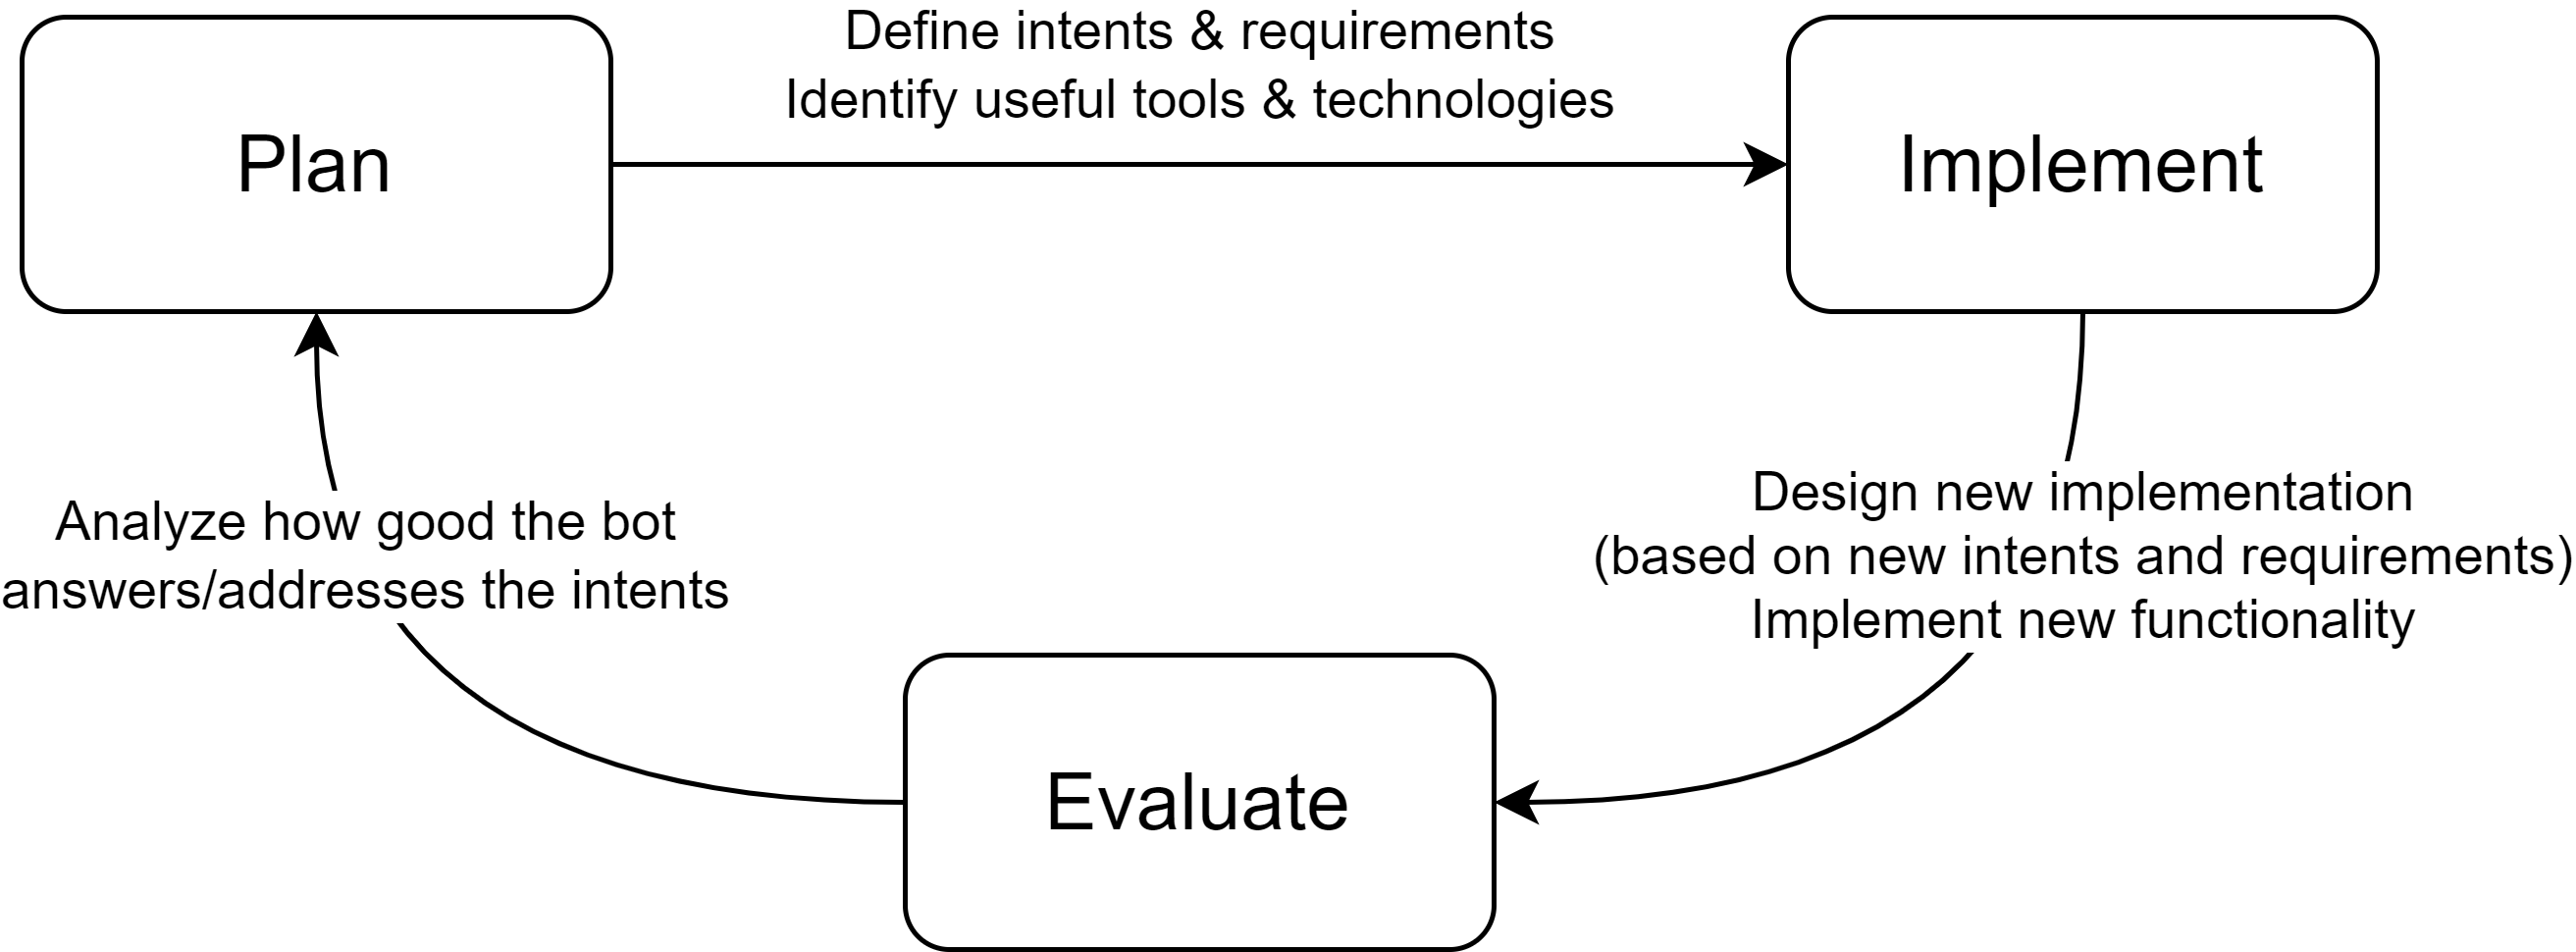
\includegraphics[width=0.95\textwidth]{graphics/iterative-design.png}
\caption{Visualization of the iterative development process.}
\label{fig:iterative-design}
\end{figure}
The research methodology for this thesis is splitted into two phases, with the first one focusing on a comprehensive literature review.
In this initial step existing concepts and building blocks for chatbot development will be gathered to provide a foundation for understanding how to develop an intelligent chatbot.
Additionally, the literature review should provide prior work that developed chatbots with similar functionalities even if in other domains.
This analysis should help to identify insights and best practices transferable for the implementation of a chatbot tailored to smart home applications.

The second key phase of the methodology involves an iterative development process to create an example architecture and chatbot prototype. 
This process is shown in \cref{fig:iterative-design}.
During the planning stage, the research defines useful intents and requirements essential for the chatbot's functionality. 
This stage also includes the identification of valuable tools and technologies, along with strategies for making the necessary data accessible to the chatbot.

The subsequent implementation phase involves the analysis and design of a new implementation based on the identified intents and requirements. This step aims to construct a chatbot architecture that aligns with the specific needs of answering complex questions within the smart home domain.

Lastly, the methodology includes a robust evaluation process to assess the perfromance of the chatbot prototype. 
This evaluation is also part of the iterative process and focuses on answering how effectively the chatbot addresses the predefined intents and requirements, providing valuable insights into its performance and areas for potential refinement. 

% todo Result
The potential result of the thesis is the development and evaluation of a chatbot for smart home systems, enhancing system explainability and user interaction. 
The research outcome offers valuable insights into the feasibility, challenges, and performance of such a chatbot, providing a foundation for future chatbots with similar use-cases.

% Conclusion
In conclusion, this thesis investigates how far a chatbot can go in addressing complex user queries to provide enhanced system explainability and user-centric functionalities.
The research outcomes underscore the potential of such chatbots while simultaneously unveiling challenges that can occur in the development process.
The findings showcase the ability of the chatbot to enhance user understanding and engagement within the smart home domain. 
The study not only contributes to the field of smart home technologies but could also act as a contact point for future innovations, where chatbots are used for intuitive and comprehensible interaction between users and their systems.

% Contributions [explicit]
\section*{Explicit Contributions}
The thesis contributes to the field of smart home technologies by developing a chatbot for home automation systems, exemplary into the Bosch Smart Home system, focusing on enhancing system explainability and addressing user-centric functionalities. 
It provides a novel exploration of chatbot architectures, tools, and methodologies that could be used for answering complex questions within smart home environments. 
The research provides insights into potential challenges of implementing such a chatbot, assesses its capabilities, and offers recommendations for future developments. 
Ultimately, this thesis aims to give users a deeper understanding of their smart homes and enhance transparency and usability of home automation systems.
\section{Objective}

\section{Methodology}

\section*{Thesis Structure}
Here, give an overview of your thesis structure.
\begin{description}
\item[Chapter~\ref{chap:evaluation} -- \nameref{chap:evaluation}:] Here, we provide...
\item[Chapter~\ref{chap:conclusion} -- \nameref{chap:conclusion}] We conclude our thesis ...
\end{description}
